\documentclass[a4paper, 12pt]{report}

% load packages
%\usepackage{showframe}
\usepackage[utf8]{inputenc}
\usepackage{graphicx}
\usepackage[export]{adjustbox}
\usepackage{float}

\begin{document}

\title{Quick Start Guide of Project 1 for CS 6360.0U1 - Database Design}

\author{Siming Liu}

\maketitle{}

\noindent There are five categories of operations described one by one below.

\section*{Branch Selection}

Once the program is started, the branch selection windows is automatically opened. Librarians could use this window to selection corresponding branch.
\begin{figure}[H]
  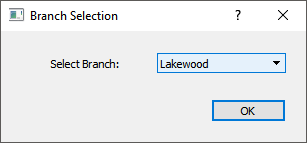
\includegraphics[scale=0.8]{./screenshot/branch_selection.png}
  \caption{Branch Selection}
\end{figure}

\pagebreak

\section*{Searching Book}
To search a book, just simply input keywords in the searching frame. Please separate them by \textbf{spaces}.
\begin{figure}[H]
  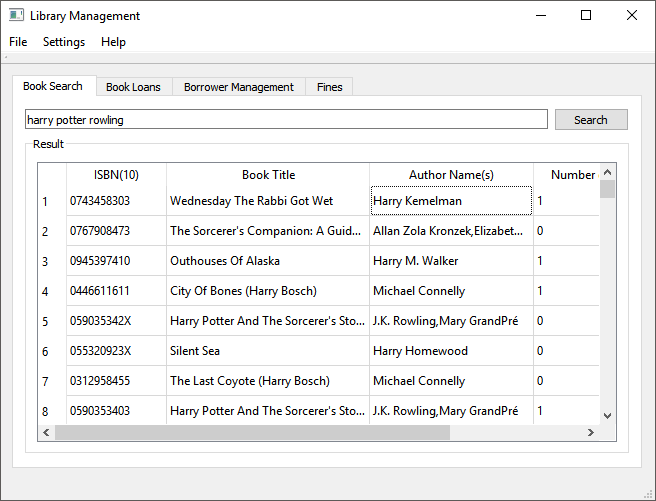
\includegraphics[width=\textwidth, inner]{./screenshot/searching.png}
  \caption{Searching}
\end{figure}

\pagebreak

\section*{Checking out}
To check out a book, just simply input \textbf{Book ID} and \textbf{Card Number}. Then press button \textit{Check out}. If the reader could successfully check out this book, a dialog will pop up and the result record will show in the below frame. If the reader could not check out a book due to overdue or fines, some corresponding dialog will show to indicate the problem.
\begin{figure}[H]
  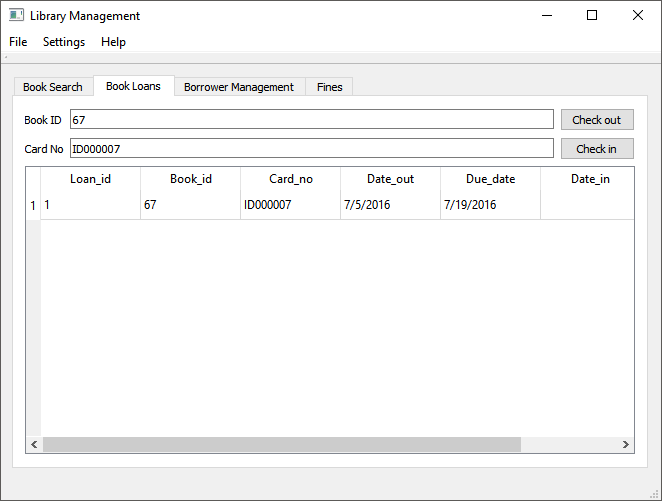
\includegraphics[width=\textwidth, inner]{./screenshot/checking_out.png}
  \caption{Checking out}
\end{figure}

\pagebreak

\section*{Checking in}
Checking in shares the same tab with checking out. To check in a book, just simply input \textbf{Book ID}. Then press button \textit{Check in}. If the reader has any overdue, a dialog will show to indicate that. Otherwise, the result will show in the below frame.
\begin{figure}[H]
  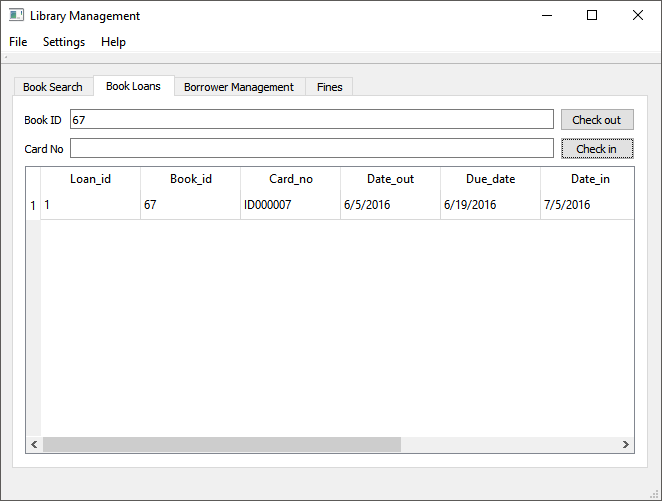
\includegraphics[width=\textwidth, inner]{./screenshot/checking_in.png}
  \caption{Checking in}
\end{figure}

\pagebreak

\section*{Borrower Management}
To create a new borrower for the library, input corresponding information in each field. Then press button \textit{Create}. The result tuple will show in the below frame. Press button \textit{Clear} will clear all the texts in all fields.
\begin{figure}[H]
  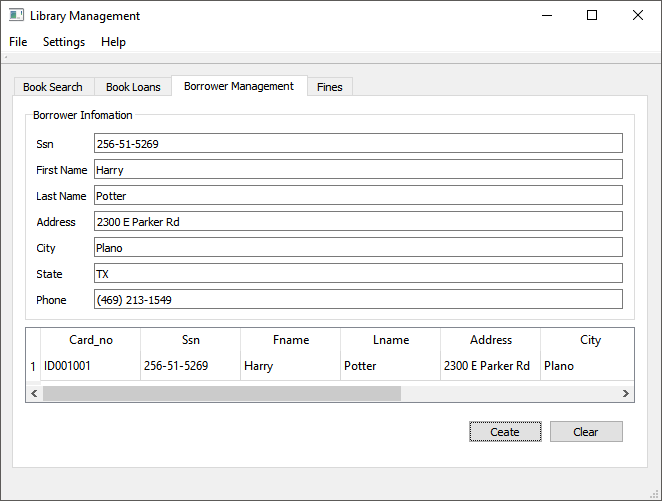
\includegraphics[width=\textwidth, inner]{./screenshot/borrower.png}
  \caption{Borrower Management}
\end{figure}

\pagebreak

\section*{Fines}
To check overdue information and fines records, simply input \textbf{Card Number} and then press button \textit{Search}. The result will show in the below two frames.

To edit fine amount and pay status, just modify the value in the frame, the result will write back to database automatically.

\begin{enumerate}
  \item For pay status, only allow to input two strings: \textbf{Paid} or \textbf{Unpaid}.
  \item For fine amount, the program only support \textbf{two} number of digits to the right of the decimal point.
\end{enumerate}

\begin{figure}[H]
  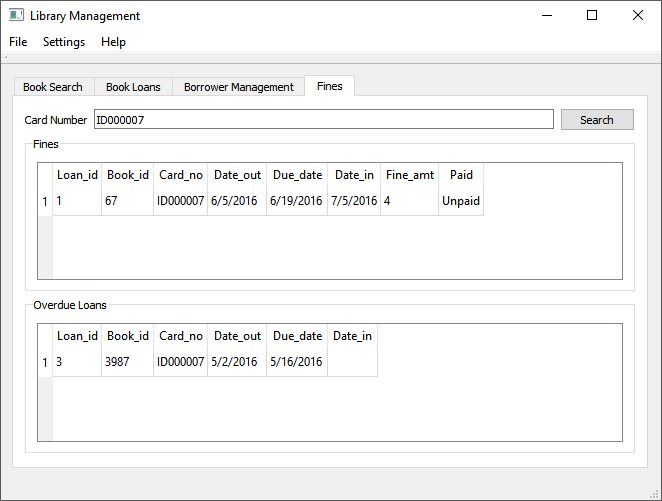
\includegraphics[width=\textwidth, inner]{./screenshot/fines.png}
  \caption{Fines}
\end{figure}

\end{document}
